\section{Testing}

For the testing of the project, \texttt{NodeRed}\cite{NodeRED} was used. This application 
allows for block-based programming and it's mainly focused on fast development for data pipelining and high level testing.

In this project, this tool was used to simulate the nodes and all the traffic sent by MQTT. The main flow constantly sends 
telemetry and for the validation, event are inserted manually. The flow can be seen in \autoref{fig:validationFlow}.
\begin{figure}[H]
    \centering
    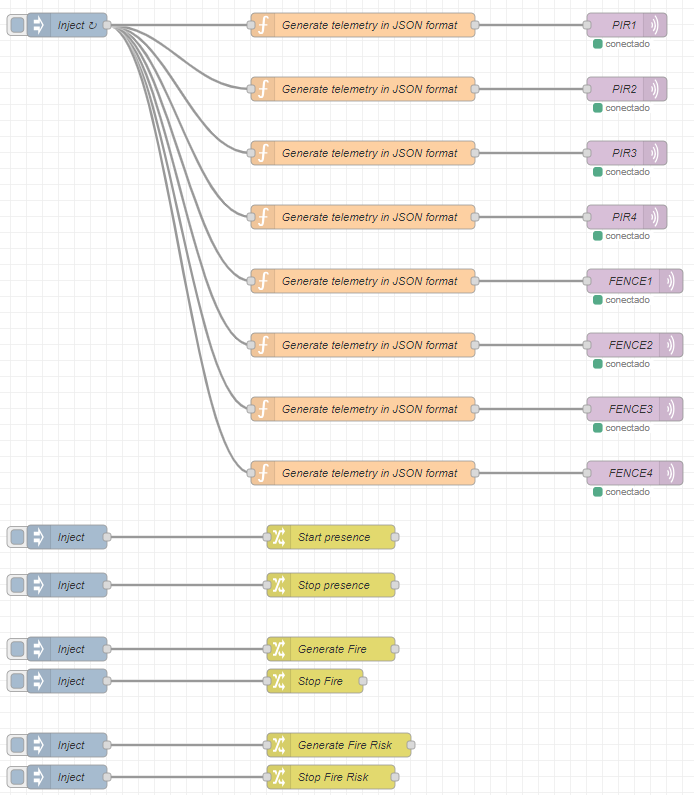
\includegraphics[width=0.7\textwidth]{./images/9/NodeRed.png}
    \caption{NodeRed Validation Flow}
    \label{fig:validationFlow}
\end{figure}

This tool was used to:
\begin{itemize}
    \item Test the best format for the traffic of the nodes.
    \item Constantly check the correct implementation of the functionalities.
    \item Insert alarms in the system to further implement new functionalities in the dashboard.
\end{itemize}

Finally, the debug utility of ThingsBoard was well used in order to test insertion of data and other conditions. This ensures that the system is 
built in a more robust manner.

